\chapter{Introducere}

\acrlong{iot} este unul din subiectele de cel mai mare interes în sfera tehnologiei,
alături de inteligența artificială, tehnologia blockchain și realitatea virtuală. 
Definiția exactă a acestui termen variază semnificativ atât în lucrările
științifice cât și în presă sau publicațiile companiilor din domeniul tehnologiei informației sau domenii adiacente. Prima dată utilizat de Kevin Ashton într-o prezentare ținută pentru Procter \& Gamble în anul 1999 \cite{ashton_2009}, acesta se referea la dispozitivele care cu ajutorul senzorilor dau capacitatea computerelor de a "vedea", "auzi" și "simți" mediul înconjurător. Astăzi, atunci când vorbim de \acrshort{iot} înglobăm o gamă largă de concepte și dispozitive: rețele wireless, electrocasnice inteligente, automatizări rezidențiale sau industriale, vehicule autonome, toate se pot încadra sub eticheta \acrshort{iot}.

Probabil cea mai răspândită și populară aplicare a sistemelor \acrshort{iot} sunt locuințele inteligente. Datorită interesului crescut pentru eficientizarea consumului de energie, reducerea emisiilor de carbon, dar și al beneficiilor promise pentru calitatea vieții, locuințele și orașele inteligente interconectate prin internet au devenit un vis tehnologic atât al cetățenilor cât și al companiilor sau guvernelor. De la iluminare cu senzori de mișcare până la asistenți virtuali care ne învață preferințele legate de muzică sau temperatură, suntem tot mai înconjurați de \textit{lucruri} (\textit{things}) inteligente, interconectate, ce procesează cantități enorme de date despre mediul nostru, dar și despre noi. 

Deși este o nișă relativ tânără, rețelele de dispozitive inteligente își fac loc în tot mai multe industrii și domenii de activitate cu o lungă istorie. În fabricile moderne se utilizează rețele complexe de senzori, roboți și dispozitive de coordonare pentru a facilita linii de producție. În agricultură atât monitorizarea cât și îngrijirea culturilor se poate realiza folosind senzori și drone conectate la internet. În sectorul public există inițiative de digitalizare a infrastructurii și comunicării dintre instituții și cetățeni, scopul final fiind crearea de orașe cu adevărat inteligente. 

Considerând importanța contextului prezentat, lucrarea de față își propune să analizeze metodele existente de testare a sistemelor \acrshort{iot}, în principal aspectele funcționale, dar cu un interes aparte pentru una din proprietățile nefuncționale, și anume securitatea. Pe lângă analiza teoretică a literaturii și practicilor existente, voi include rezultate experimentale obținute atât prin reproducerea experimentelor din literatură, cât și ale abordărilor proprii.

Capitolul curent conține în secțiunile ce urmează o analiză detaliată a motivației și interesului pentru îmbunătățirea tehnicilor de testare a sistemelor \acrshort{iot}, un scurt istoric al domeniului, un sumar al contribuțiilor prezentate, iar în final o prezentare a structurii și conținutului prezentei lucrări.

\section{Motivația pentru temă}

M-am alăturat echipei de cercetare a proiectului \textit{\acrfull{sasha}} realizat de Universitatea din București în colaborare cu Universitatea Politehnică din București, motivat fiind de provocarea de a explora securitatea sistemelor informatice într-o arie relativ tânără a tehnologiei, în care lipsesc practicile consacrate. Am avut astfel oportunitatea de a înțelege provocările și obstacolele întâlnite în dezvoltarea aplicațiilor \acrshort{iot}, în particular a celor pentru locuințe inteligente, de a lua la cunoștință soluțiile și practicile existente, iar mai apoi am putut contribui la realizarea unui articol de cercetare (TODO: de citat articolul cand o avea DOI), anume \textit{Building blocks for IoT testing - a benchmark of IoT apps and a functional testing framework}, care dorește să îmbunătățească metodele de evaluare și comparare al tehnicilor de testare din \acrlong{iot}.

Pentru a fructifica experiența obținută în urma colaborării, am decis să realizez o lucrare care să înglobeze întreaga mea contribuție, oferindu-i contextul necesar pentru o bună înțelegere. 

\section{Scurt istoric al Internet of Things}

% todo: de citat surse

Conceptul de dispozitive interconectate există încă din timpul apariției telegrafului, însă primele inițiative cu adevărat moderne le întâlnim abia în anii 1980 - 1990. Prima discuție cu urmări practice despre dispozitive inteligente conectate într-o rețea apare în 1982, când studenții de la  Carnegie Mellon University au folosit un tonomat Coca-Cola modificat conectat la \textit{ARPANET} (precursorul internetului modern) pentru a raporta automat inventarul și încasările. În decursul a puțini ani, lucrări precum \cite{Weiser1999}, dar și alte publicații de presă sau academice au conturat viziunea despre dispozitivele interconectate și interacțiunea lor cu viețile noastre. \cite{Raji1994} descrie în abstractul lucrării sale rețelele inteligente astfel (tradus din engleză):

% Control networks move small packets of data to a large set of nodes, so as to integrate and automate everything from home appliances to entire factories

\say{Rețelele de control transportă pachete mici de date la un număr mare de noduri, astfel integrând și automatizând totul de la aparate casnice până la întregi fabrici. {[}...{]}}

În anii următori, numeroase companii precum Microsoft, Novell sau LG au dezvoltat produse și soluții formate din mai multe dispozitive interconectate. Termenul de \acrlong{iot} devine consacrat abia în 1999, așa cum am menționat anterior, datorită lui Kevin Ashton însă va mai dura încă zece ani până la o creștere considerabilă a popularității.

În anul 2011, \cite{Gartner2011} include \acrlong{iot} pe lista tehnologiilor \textit{on the rise}, iar conforma \cite{statistaIot} valora 300 de miliarde de dolari. Astăzi, valorează de aproape șase ori mai mult, 1.700 de miliarde de dolari, iar conform Google Trends este într-o explozivă creștere a popularității după anul 2015.

Astăzi, \acrlong{iot} este unul din cele mai populare subiecte atât în presa, în publicații precum Forbes sau The Economist, cât și în mediul academic, fiind publicate din 2010 peste 400 de articole doar despre asigurarea calității în IoT conform \cite{Ahmed2019}.

% TODO: sa mai cizelez un pic istoricul

\begin{figure}[h]
\caption{Statistici Google Trends pentru Internet of Things din 2004 până în prezent}
\centering
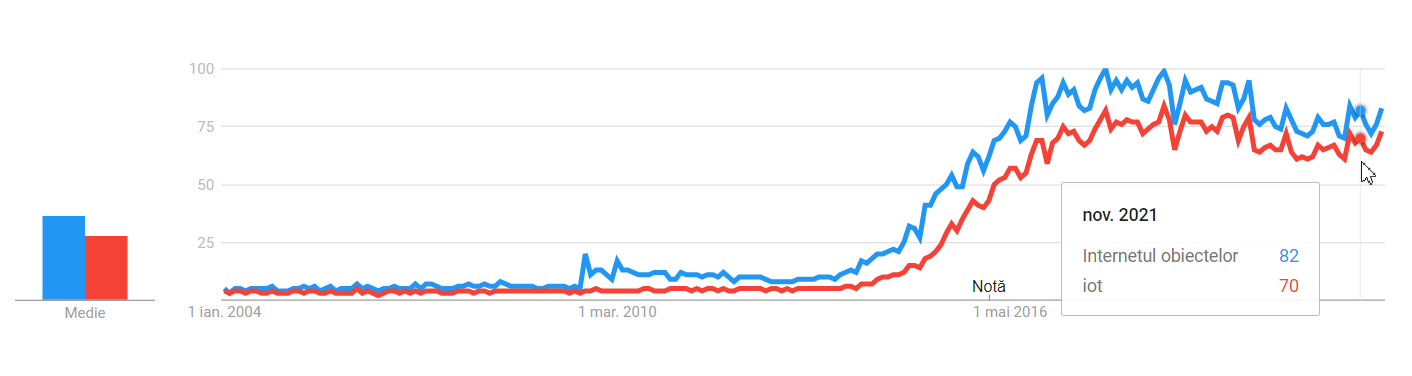
\includegraphics[width=\textwidth]{images/trends_iot.png}
\end{figure}


\section{Structura lucrării}

Capitolul curent a oferit o perspectivă de ansamblu asupra motivației, scopului și temei lucrării. În cele ce urmează, capitolul 2 va prezenta noțiunile necesare pentru înțelegerea lucrării, oferind o serie de definiții, uneori proprii, pentru termenii utilizați, o analiză amănunțită a literaturii existente despre testarea sistemelor IoT urmărind să definească obiectivele. Capitolul 3 conține o descriere atât teoretică, cât și tehnică a sistemelor IoT, oferind definiții riguroase și exemple. Atenție suplimentară va fi acordată locuințelor inteligente într-un studiu de caz dedicat, deoarece acestea au servit ca principal model pentru realizarea experimentelor. În capitolul 4 găsim motivația pentru realizarea unui set de aplicații de evaluare pentru tehnicile de testare și descrierea implementării tehnice a unui astfel de \textit{benchmark}. Capitolul 5 continuă prin evaluarea unor tehnici de testare funcțională pe setul de aplicații propus anterior, iar capitolul 6 se concentrează pe evaluarea eficienței tehnicilor ce folosesc \textit{fuzzing}. În final, capitolul 7 oferă concluziile lucrării, fiind urmat de glosarul termenilor și bibliografie.